% VLDB template version of 2020-08-03 enhances the ACM template, version 1.7.0:
% https://www.acm.org/publications/proceedings-template
% The ACM Latex guide provides further information about the ACM template

\documentclass[sigconf, nonacm, pdfa]{acmart}

%% The following content must be adapted for the final version
% paper-specific
\newcommand\vldbdoi{XX.XX/XXX.XX}
\newcommand\vldbpages{XXX-XXX}
% issue-specific
\newcommand\vldbvolume{18}
\newcommand\vldbissue{9}
\newcommand\vldbyear{2025}
% should be fine as it is
\newcommand\vldbauthors{\authors}
\newcommand\vldbtitle{\shorttitle} 
% leave empty if no availability url should be set
\newcommand\vldbavailabilityurl{https://github.com/wzzzzd/pathce}
% whether page numbers should be shown or not, use 'plain' for review versions, 'empty' for camera ready
\newcommand\vldbpagestyle{empty} 
 
% Enumerate and Itemize modifications
\usepackage[a-2b]{pdfx}
\usepackage{multirow}
\usepackage{graphicx} % Required for inserting images
\usepackage{subcaption}% Offers an user interface to sub-captions.
\usepackage{float}% Improves the interface for defining floating objects

\usepackage{enumitem}
\usepackage{xspace}
\usepackage{multirow}
\usepackage{amsmath} %maths
\let\Bbbk\relax
\usepackage{amssymb} %maths
%\usepackage[right,inline]{showlabels}
%\renewcommand{\showlabelfont}{\small\color{red}}
\usepackage[ruled, linesnumbered, noend]{algorithm2e}
\usepackage{listings}

\usepackage[tableposition=top]{caption}
\captionsetup{textfont={normalfont}}
\definecolor{dkgreen}{rgb}{0,0.6,0}
\definecolor{gray}{rgb}{0.5,0.5,0.5}
\definecolor{mauve}{rgb}{0.58,0,0.82}
\usepackage{subcaption}
\usepackage{relsize}
\usepackage{stfloats}
\newcommand*{\defeq}{\stackrel{\mathsmaller{\mathsf{def}}}{=}}
\setlist{topsep=0pt,noitemsep} \setitemize[1]{label=$\circ$}
%%%%%%%%%%%%%%%%%%%%%%%%%%%%%%%%%%%%%%%%%%%

\sloppy

\newcommand{\rtable}[1]{\ensuremath{\mathsf{#1}}}
\newcommand{\ratt}[1]{\ensuremath{\mathit{#1}}}
\newcommand{\at}[1]{\protect\ensuremath{\mathsf{#1}}\xspace}
\newcommand{\myhrule}{\rule[.5pt]{\hsize}{.5pt}}
\newcommand{\oneurl}[1]{\texttt{#1}}
\newcommand{\stab}{\rule{0pt}{8pt}\\[-1.2ex]}
\newcommand{\sttab}{\rule{0pt}{8pt}\\[-2.7ex]}
\newcommand{\sstab}{\rule{0pt}{8pt}\\[-1.8ex]}
\newcommand{\tabstrut}{\rule{0pt}{4pt}\vspace{-0.07in}}
\newcommand{\vs}{\vspace{1ex}}
\newcommand{\exa}[2]{{\tt
    \begin{tabbing}\hspace{#1}\=\+\kill #2
\end{tabbing}}}
\newcommand{\ra}{\rightarrow}
\newcommand{\Ra}{\Rightarrow}
\newcommand{\la}{\leftarrow}
\newcommand{\bi}{
\begin{itemize}}
    \newcommand{\ei}{
  \end{itemize}}
\newenvironment{tbi}{
  \begin{itemize}
    \setlength{\topsep}{0.6ex}\setlength{\itemsep}{0ex}} %\vspace{-0.5ex}}
    {
  \end{itemize}} %\vspace{-0.5ex}}
\newenvironment{tbe}{
  \begin{enumerate}
    \setlength{\topsep}{0ex}\setlength{\itemsep}{0ex}\vspace{0ex}}
    {
  \end{itemize}\vspace{-1ex}}

\newcommand{\mat}[2]{{
    \begin{tabbing}\hspace{#1}\=\+\kill #2
\end{tabbing}}}
\newcommand{\m}{\hspace{0.05in}}
\newcommand{\ls}{\hspace{0.1in}}
\newcommand{\be}{
\begin{enumerate}}
    \newcommand{\ee}{
  \end{enumerate}}
%\newcommand{\beqn}{\begin{eqnarray*}}
%\newcommand{\eeqn}{\end{eqnarray*}}
\newcommand{\beqn}{
\begin{eqnarray}}
  \newcommand{\eeqn}{
\end{eqnarray}}

\newcommand{\card}[1]{\mid\! #1\!\mid}
\newcommand{\fth}{\hfill $\Box$}
\newcommand{\AND}{\displaystyle{\bigwedge_{i=1}^{n}}}
%\newcommand{\U}[1]{\displaystyle{\bigcup_{#1}}}
\newcommand{\Sm}[1]{\displaystyle{\sum_{#1}}}
\newcommand{\stitle}[1]{\vspace{1.6ex}\noindent{\bf #1}}
\newcommand{\etitle}[1]{\vspace{1ex}\noindent{\underline{\em #1}}}
\newcommand{\eetitle}[1]{\vspace{0.8ex}\noindent{{\em #1}}}
\renewcommand{\t}{\tau}
\newcommand{\Inh}[1]{\$#1}
\renewcommand{\r}[1]{{\it rule}(#1)}
\newcommand{\pa}{\parallel}
\newcommand{\LHS}{\kw{{\small LHS}}\xspace}
\newcommand{\RHS}{\kw{RHS}\xspace}
\newcommand{\ie}{\emph{i.e.,}\xspace}
\newcommand{\eg}{\emph{e.g.,}\xspace}
\newcommand{\wrt}{\emph{w.r.t.}\xspace}
\newcommand{\aka}{\emph{a.k.a.}\xspace}
\newcommand{\kwlog}{\emph{w.l.o.g.}\xspace}
\newcommand{\st}{\emph{s.t.}\xspace}
%%%%%%%%%%%%%%%%%%%%%%%%%%%%%%%%%%%%%%%%%%%%%%%%%%%%%%%%%%%%%%%%
%                  Relation Algebra operators
%%%%%%%%%%%%%%%%%%%%%%%%%%%%%%%%%%%%%%%%%%%%%%%%%%%%%%%%%%%%%%%%

\newcommand{\RS}{{\small S}\xspace}
\newcommand{\RP}{{\small P}\xspace}
\newcommand{\RJ}{{\sc j}\xspace}
\newcommand{\RC}{{\small C}\xspace}
\newcommand{\RSJ}{{\small SJ}\xspace}
\newcommand{\RSC}{{\small SC}\xspace}
\newcommand{\RSP}{{\small SP}\xspace}
\newcommand{\RPJ}{{\small PJ}\xspace}
\newcommand{\RPC}{{\small PC}\xspace}
\newcommand{\RSPJ}{{\sc spj}\xspace}
\newcommand{\RSPC}{{\small SPC}\xspace}
\newcommand{\RSPJU}{{\sc spju}\xspace}
\newcommand{\RSPCU}{{\small SPCU}\xspace}
\newcommand{\RSPJUN}{{\small SPJU$^N$}\xspace}
\newcommand{\RSPCUN}{{\small SPCU$^N$}\xspace}
%%%%%%%%%%%%%%%%%%%%%%%%%%%%%%%%%%%%%%%%%%%%%%%%%%%%%%%%%%%%%%%%%%%%%%%%%%%%%%
% ALGORITHMS
%%%%%%%%%%%%%%%%%%%%%%%%%%%%%%%%%%%%%%%%%%%%%%%%%%%%%%%%%%%%%%%%%%%%%%%%%%%%%%%
% \newcommand{\SELECT}{\mbox{{\bf select}}\ }
% \newcommand{\FROM}{\mbox{{\bf from}\ }}
% \newcommand{\WHERE}{\mbox{\bf where}\ }
% \newcommand{\SUM}{\mbox{{\bf sum}}\ }
% \newcommand{\GROUPBY}{\mbox{{\bf group by}}\ }
% \newcommand{\HAVING}{\mbox{{\bf having}}\ }
% \newcommand{\CASE}{\mbox{{\bf case}}\ }
% \newcommand{\END}{\mbox{{\bf end}}\ }
% \newcommand{\WHEN}{\mbox{{\bf when}}\ }
% \newcommand{\EXISTS}{\mbox{{\bf exists}}\ }
% \newcommand{\COUNT}{\mbox{\kw{count}}}
% \newcommand{\INSERTINTO}{\mbox{{\bf insert into}}\ }
% \newcommand{\UPDATE}{\mbox{{\bf update}}\ }
% \newcommand{\SET}{\mbox{{\bf set}}\ }
% \newcommand{\IN}{\mbox{{\bf in}}\ }
% \newcommand{\If}{\mbox{\bf if}\ }
% \newcommand{\Let}{\mbox{\bf let}\ }
% \newcommand{\Call}{\mbox{\bf call}\ }
% \newcommand{\Then}{\mbox{\bf then}\ }
% \newcommand{\To}{\mbox{\bf to}\ }
% \newcommand{\Else}{\mbox{\bf else}\ }
% \newcommand{\ElseIf}{\mbox{\bf elseif}\ }
% \newcommand{\While}{\mbox{\bf while}\ }
% \newcommand{\Begin}{\mbox{\bf begin}\ }
% \newcommand{\End}{\mbox{\bf end}\ }
% \newcommand{\Do}{\mbox{\bf do}\ }
% \newcommand{\Downto}{\mbox{\bf downto}\ }
% \newcommand{\Repeat}{\mbox{\bf repeat}\ }
% \newcommand{\Until}{\mbox{\bf until}\ }
% \newcommand{\For}{\mbox{\bf for}\ }
% \newcommand{\Each}{\mbox{\bf each}\ }

% \newcommand{\ForEach}{\mbox{\bf for each}\ }
% \newcommand{\Or}{\mbox{\bf or}\ }
% \renewcommand{\And}{\mbox{\bf and}\ }
% \newcommand{\Not}{\mbox{\bf not}\ }
% \newcommand{\Break}{\mbox{\bf break}\ }
% \newcommand{\Continue}{\mbox{\bf continue}\ }
% \newcommand{\Return}{\mbox{\bf return}\ }
% \newcommand{\Case}{\mbox{\bf case}\ }
% \newcommand{\Of}{\mbox{\bf of}\ }
% \newcommand{\EndCase}{\mbox{\bf end-case}\ }
% \newcommand{\NIL}{\mbox{\em nil}}
% \newcommand{\False}{\mbox{\em false}\xspace}
% \newcommand{\True}{\mbox{\em true}\xspace}
% \newcommand{\algAND}{{\sc and}\xspace}
% \newcommand{\OR}{{\sc or}\xspace}
% \newcommand{\NOT}{{\sc not}\xspace}
\newcommand{\kw}[1]{{\ensuremath {\mathsf{#1}}}\xspace}
\newcommand{\Reps}{S}
\newcounter{ccc}
\newcommand{\bcc}{\setcounter{ccc}{1}\theccc.}
\newcommand{\bccc}{\theccc.}
\newcommand{\icc}{\addtocounter{ccc}{1}\theccc.}
\newcommand{\checking}{{\mbox{\small\sf Checking}\xspace}}
\newcommand{\preProcessing}{{\mbox{\small\sf preProcessing}\xspace}}
\newcommand{\CFDconsistency}{{\mbox{\small\sf CFD\_Checking}\xspace}}
\newcommand{\MCS} {\kw{MCS}}
\newcommand{\EIP} {\kw{EIP}}
\newcommand{\CDP} {\kw{DMP}}
\newcommand{\templateDB}{{\mbox{\small\sf templateDB}\xspace}}
\newcommand{\ChaseChecking}{{\mbox{\small\sf RandomChecking}\xspace}}
\newcommand{\chase}{{\mbox{\small\sf Chase}\xspace}}
\newcommand{\deduced}{\kw{deduced}}
\newcommand{\deducedD}{\kw{deduced}_\Delta}
\newcommand{\deducedDP}{\kw{deduced}_{\Delta}^{+}}
\newcommand{\deducedDM}{\kw{deduced}_{\Delta}^{-}}
\newcommand{\SAT}{{\mbox{\small\sf SAT}\xspace}}
\newcommand{\kSAT}{{\mbox{\small 3SAT}\xspace}}
\newcommand{\PropCFDSPC}{\kw{Prop{\small CFD\_SPC}}}
\newcommand{\PropCFDSPCU}{\kw{Prop{\small CFD\_SPCU}}}
\newcommand{\UnionEQs}{\kw{UnionEQs}}
\newcommand{\UnionCFDs}{\kw{UnionCFDs}}
\newcommand{\EQ}{\kw{EQ}}
\newcommand{\eq}{\kw{eq}}
\newcommand{\key}{\kw{key}}
\newcommand{\rep}{\kw{rep}}
\newcommand{\PEQ}{\kw{EQ2CFD}}
\newcommand{\Drop}{\kw{Drop}}
\newcommand{\Res}{\kw{Res}}
\newcommand{\CFD}{{\small CFD}\xspace}
\newcommand{\CFDs}{{\small CFD}{\small s}\xspace}
\newcommand{\CIND}{{\sc cind}\xspace}
\newcommand{\cind}{{\small \sf CIND}}
\newcommand{\cfd}{{\small \sf CFD}}
\newcommand{\CINDp}{{\sc cind}$^+$\xspace}
\newcommand{\CINDn}{{\sc cind}$^-$\xspace}
\newcommand{\CINDs}{{\sc cind}{\small s}\xspace}
\newcommand{\FD}{\kw{FD}}
\newcommand{\FDs}{\kw{FDs}}
\newcommand{\IND}{{\sc ind}\xspace}
\newcommand{\INDs}{{\sc ind}{\small s}\xspace}
\newcommand{\TGDs}{\kw{TGDs}}
\newcommand{\NP}{\kw{NP}}
\newcommand{\DP}{\kw{DP}}
\newcommand{\DAGs}{{\small DAG}s\xspace}
\newcommand{\NC}{{\sc nc}\xspace}
\newcommand{\coNP}{\kw{coNP}}
\newcommand{\PTIME}{\kw{PTIME}}
\newcommand{\PSPACE}{{\sc pspace}\xspace}
\newcommand{\EXPTIME}{{\sc exptime}\xspace}
\newcommand{\NPSPACE}{{\sc npspace}\xspace}
\newcommand{\dom}{\protect\ensuremath{\mathsf{dom}}\xspace}
\newcommand{\atset}{\protect\ensuremath{\mathsf{attr}}\xspace}
\newcommand{\attr}[1]{\protect\ensuremath{\mathsf{#1}}\xspace}
\newcommand{\attrset}{\protect\ensuremath{\mathsf{attr}}\xspace}
\newcommand{\finatset}{\protect\ensuremath{\mathsf{finattr}}\xspace}
\newcommand{\pvar}{\protect\ensuremath{\mathsf{var\%}}\xspace}
\newcommand{\lLHS}{\protect\ensuremath{\mathsf{{\small LHS}}}\xspace}
\newcommand{\RA}{{\small RA}\xspace}
\newcommand{\RBR}{\kw{RBR}}
\newcommand{\SQL}{{\sc sql}\xspace}
\newcommand{\XSLT}{{\sc xslt}\xspace}
\newcommand{\DBMS}{{\sc dbms}\xspace}
\newcommand{\ATG}{{\sc atg}\xspace}
\newcommand{\ATGs}{{\sc atg}{\small s}\xspace}
\newcommand{\EBI}{{\sc ebi}\xspace}
\newcommand{\GO}{{\sc go}\xspace}
\newcommand{\VEC}[1]{{\sc vec}(#1)}
\newcommand{\DAG}{{\small DAG}\xspace}
\newcommand{\XQ}{{\sc xq}\xspace}
\newcommand{\XQwc}{{\sc xq}$^{\scriptscriptstyle[*]}$\xspace}
\newcommand{\XQdes}{{\sc xq}$^{\scriptscriptstyle[//]}$\xspace}
\newcommand{\XQfull}{{\sc xq}$^{\scriptscriptstyle[*,//]}$\xspace}
\newcommand{\vect}[1]{$\langle$ #1 $\rangle$}
\newcommand{\sem}[1]{[\![#1]\!]}
\newcommand{\NN}[2]{#1\sem{#2}}
\newcommand{\e}[2]{{\mathit (#1,#2)}}
\newcommand{\ep}[2]{{\mathit (#1,#2)+}}
\newcommand{\brname}{\ensuremath{{\mathsf{N}}}}
\newcommand{\budrel}[1]{\ensuremath{{\brname_{#1}}}}
\newcommand{\budgen}[2]{\ensuremath{Q^\brname_\e{#1}{#2}}}
\newcommand{\budcut}[2]{\ensuremath{Q_\e{#1}{#2}}}
\newcommand{\R}{{\mathcal R}}
\newcommand{\A}{{\mathcal A}}
\newcommand{\B}{{\mathcal B}}
\newcommand{\Buff}[1]{{\mathbb{B}_{#1}}}
%\newcommand{\buf}[1]{{\mathbb{B}^b_{#1}}}
\newcommand{\Q}{{\mathcal Q}}
\newcommand{\Y}{{\mathcal Y}}
\newcommand{\I}{{\mathcal I}}
%\newcommand{\V}{{\mathcal V}}
%\newcommand{\E}{{\mathcal E}}
%\newcommand{\Lq}{{\mathcal L}}

\newcommand{\flag}{\kw{flag}}
\newcommand{\BF}{\kw{BF}}
\newcommand{\precision}{\kw{precision}}
\newcommand{\recall}{\kw{recall}}
\newcommand{\accuracy}{\kw{accuracy}}

\newcommand{\eop}{\hspace*{\fill}\mbox{$\Box$}}     % End of proof
\newcounter{example}%[section]
\renewcommand{\theexample}{\arabic{example}}
%\renewenvironment{example}{
\newenvironment{example}{
  \vspace{1.5ex}
  \refstepcounter{example}
{\noindent\bf Example \theexample:}}{
\eop\vspace{1.5ex}}
\def\copyrightspace{}
\renewcommand{\ni}{\noindent}
\newcommand{\comlore}[1]{
  \begin{minipage}{3in}\fbox{\fbox{\parbox[t]{3in}{{\vspace{2mm}\noindent
            \bf COMM(LORE):~
    { #1}\hfill  END.}}}}
\end{minipage}\\}
\newcommand{\comwenfei}[1]{
  \begin{minipage}{3in}\fbox{\fbox{\parbox[t]{3in}{{\vspace{2mm}\noindent
            \bf COMM(WENFEI):~
    { #1}\hfill  END.}}}}
\end{minipage}\\}
\newcommand{\comshuai}[1]{
  \begin{minipage}{3in}\fbox{\fbox{\parbox[t]{3in}{{\vspace{2mm}\noindent
            \bf COMM(SHUAI):~
    { #1}\hfill  END.}}}}
\end{minipage}\\}
\newcommand{\nthesection}{\arabic{section}}
\newcounter{theorem}
%\renewcommand{\thetheorem}{\arabic{theorem}}
%\newcommand{\thetheorem}{\arabic{theorem}}
\newcounter{prop}
\renewcommand{\theprop}{\arabic{theorem}}
\newcounter{lemma}
\renewcommand{\thelemma}{\arabic{theorem}}
\newcounter{cor}
\renewcommand{\thecor}{\arabic{theorem}}
%\renewenvironment{theorem}{\begin{em}
\newenvironment{theorem}{
  \begin{em}
    \refstepcounter{theorem}
  {\vspace{1.5ex} \noindent\bf  Theorem  \thetheorem:}}{
\end{em}\eop\vspace{1.5ex}} %\hspace*{\fill}\vspace*{1ex}}
\newenvironment{ctheorem}[1]{
  \begin{em}
    \refstepcounter{theorem}
  {\vspace{1ex}{\noindent \bf Theorem  \thetheorem~[#1]}: }}{
\end{em}\eop\vspace{1.5ex}}
%\hspace*{\fill}\mbox{$\Box$}\vspace*{1.5ex}}
\newenvironment{prop}{
  \begin{em}
    \refstepcounter{theorem}
  {\vspace{1.5ex}\noindent \bf Proposition \theprop:}}{
\end{em}\eop\vspace{1.5ex}}%\hspace*{\fill}\vspace*{1ex}}
\newenvironment{propx}{
  \begin{em}
    \refstepcounter{theorem}
  {\vspace{1.5ex}\noindent \bf Proposition \theprop:}}{
\end{em}}
\newenvironment{lemma}{
  \begin{em}
    \refstepcounter{theorem}
  {\vspace{1ex}\noindent\bf Lemma \thelemma:}}{
\end{em}\eop\vspace{1ex}} %\hspace*{\fill}\vspace*{1ex}}
\newenvironment{cor}{
  \begin{em}
    \refstepcounter{theorem}
  {\vspace{1.5ex}\noindent\bf Corollary \thecor:}}{
\end{em}\eop\vspace{1.5ex}} %\hspace*{\fill}\vspace*{1ex}}
\newcounter{definition}[section]
\renewcommand{\thedefinition}{\nthesection.\arabic{definition}}
%\renewenvironment{definition}{
\newenvironment{definition}{
  \vspace{1.5ex}
  \refstepcounter{definition}
{\noindent\bf Definition {\bf \thedefinition}:}}{\eop\vspace{1.5ex}
}
\newenvironment{definitionx}{
  \vspace{1.5ex}
  \refstepcounter{definition}
{\noindent\bf Definition {\bf \thedefinition}:}}{
}
\newcounter{alg}[section]
\renewcommand{\thealg}{\nthesection.\arabic{alg}}
\newenvironment{alg}[1]{
  \refstepcounter{alg}
{\vspace{1ex}\noindent\bf Algorithm \thealg:\, #1}}{
\vspace*{1ex}}
\newcounter{arule}
\renewcommand{\thearule}{\arabic{arule}}
\newenvironment{arule}{
  \vspace{0.6ex}
  \refstepcounter{arule}
{\noindent \em Rule \thearule:}}{
}
\newcounter{claim}
\renewcommand{\theclaim}{\arabic{claim}}
\newenvironment{claim}{
  \vspace{0.6ex}
  \refstepcounter{claim}
{\noindent\em Claim \theclaim:}}{{ Wenfei Fan}\\
}
\renewenvironment{proof}{
  \vspace{1ex}
{\noindent\bf Proof:}}{\eop\vspace{1ex}}
\newenvironment{proofS}{
  \vspace{1ex}
{\noindent\bf Proof sketch:\ }}{\eop\vspace{1ex}}

%\newcommand{\SIM}{\ensuremath{\mathsf{mat}}}
\newcommand{\SIM}{\kw{SIM}}

\newcommand{\SIMe}{\ensuremath{\mathsf{mat_e}}}

\newcommand{\GPAR}{\kw{GPAR}}
\newcommand{\GPARs}{\kw{GPARs}}
\newcommand{\GRAPE}{\kw{GRAPE}}
\newcommand{\AGRAPE}{\kw{GRAPE+}}

\newcommand{\TIE}{\kw{TIE}}
\newcommand{\TIEs}{\kw{TIEs}}
\newcommand{\CFLogic}{\kw{RecLogic}}

\newcommand{\suport}{\kw{supp}}
\newcommand{\confd}{\kw{conf}}
\newcommand{\cd}[1]{|\!|{#1}|\!|}

\newcommand{\tbf}{\textbf{\textcolor{red}{X}}\xspace}
\newcommand{\qual}{\kw{qual}}
\newcommand{\MaxCard}{\kw{qualCard}}
\newcommand{\MaxSim}{\kw{qualSim}}

\newcommand{\Rees}{R_{(e,e)}}
%\newcommand{\Reps}{R_{(e,p)}}
%\newcommand{\Rpps}{R_{(p,p)}}
\newcommand{\ees}{\preceq_{(e,e)}}
%\newcommand{\eps}{\preceq_{(e,p)}}
\newcommand{\nees}{\not\preceq_{e,e}}
%\newcommand{\neps}{\not\preceq_{e,p}}
%\newcommand{\pps}{\preceq_{(p,p)}}
\newcommand{\bees}{\preceq^\mathsf{bw}_{(e,e)}}
\newcommand{\nbees}{\not\preceq^\mathsf{bw}_{(e,e)}}
%\newcommand{\beps}{\preceq^\mathsf{bw}_{(e,p)}}
%\newcommand{\nbeps}{\not\preceq^\mathsf{bw}_{(e,p)}}

\newcommand{\iees}{\precsim^{1-1}_{(e,e)}}
\newcommand{\ieps}{\precsim^{1-1}_{(e,p)}}
\newcommand{\sees}{\precsim_{(e,e)}}
%\newcommand{\seps}{\precsim^s_{(e,p)}}
\newcommand{\seps}{\precsim_{(e,p)}}
\newcommand{\nseps}{\not\precsim_{(e,p)}}
\newcommand{\nieps}{\not\precsim^{1-1}_{(e,p)}}
\newcommand{\oees}{\precsim^{\kw{opt}}_{(e,e)}}
\newcommand{\oeps}{\precsim^{\kw{opt}}_{(e,p)}}
\newcommand{\bsees}{\precsim^\mathsf{bw}_{(e,e)}}
\newcommand{\bseps}{\precsim^\mathsf{bw}_{(e,p)}}
\newcommand{\compPSim}{\kw{compPSim}}
\newcommand{\dcmp}{\kw{Dcmp}}

%\newcommand{\URL} {\kw{URL}}
%\newcommand{\URLs} {\kw{URLs}}
\newcommand{\WIS} {\kw{WIS}}
\newcommand{\IS} {\kw{IS}}
\newcommand{\AFPR}{\kw{AFP}-\kw{reduction}}
\newcommand{\AFPRs}{\kw{AFP}-\kw{reductions}}

\newcommand{\OPT}{\kw{opt}}
\newcommand{\obj}{\kw{obj}}
\newcommand{\N} {{\cal N}}
\newcommand{\kL} {{\cal L}}

\newcommand{\maxCSPS} {\kw{compMaxCard}}
\newcommand{\maxCSPI} {\kw{compMaxCard^{1-1}}}
\newcommand{\maxSSPS} {\kw{compMaxSim}}
\newcommand{\maxSSPI} {\kw{compMaxSim^{1-1}}}
\newcommand{\subIso} {\kw{cdkMCS}}
\newcommand{\combine} {\kw{combinedMaxSim}}
\newcommand{\SF}{\kw{SF}}
%\newcommand{\VSM}{\kw{VSM}}

%\newcommand{\pSim}{\kw{compSimilarity}}
\newcommand{\gSim}{\kw{graphSimulation}}

\newcommand{\maxWIS} {\kw{compMaxWIS}}
\newcommand{\nei} {\kw{Neighbor}}
\newcommand{\nonNei} {\kw{NonNeighbor}}
\newcommand{\ramsey} {\kw{Ramsey}}
\newcommand{\cRamsey} {\kw{ISRemoval}}
\newcommand{\wis} {\kw{maxWIS}}
\newcommand{\maxWeight} {\kw{maxWeight}}

\newcommand{\naive} {\kw{Naive}}
\newcommand{\good} {\kw{good}}
\newcommand{\bad} {\kw{minus}}

\newcommand{\static} {\kw{static}}
\newcommand{\parent} {\kw{prev}}
\newcommand{\child} {\kw{post}}
\newcommand{\greedy} {\kw{greedyMatch}}
\newcommand{\proNeighbor} {\kw{trimMatching}}

\newcommand{\Pick}{\mbox{\bf pick}\ }

\newcommand{\sizeof} {\kw{sizeof}}
\newcommand{\genPG} {\kw{genPGraph}}
\newcommand{\genSOL} {\kw{genSolution}}

\renewcommand{\texttt}[1]{{\small\textsf{#1}}}
\newcommand{\kchanged}{\kw{\small CHANGED}}

\definecolor{gray}{rgb}{0.5,0.5,0.5}
% \newcommand{\added}[1]{\textcolor{black}{#1}}
% \newcommand{\changed}[1]{\textcolor{red}{#1}}
% \newcommand{\removed}[1]{\textcolor{gray}{#1}}
\newcommand{\APX}{\kw{APX}-\kw{hard}}
\newcommand{\WVC}{\kw{MIN}-\kw{WVCP}}
\newcommand{\WLM}{\kw{MIN}-\kw{WLMP}}
\newcommand{\Claim}{\kw{Claim}}
\newcommand{\MWLM}{\kw{Minimum Weighted Landmark}-\kw{Cover}}
\newcommand{\problem}{\kw{Problem}}
\newcommand{\setcover}{\kw{SET}-\kw{COVER}}
\newcommand{\len}{\kw{len}}
\newcommand{\dis}{\kw{dis}}
\newcommand{\khopjoin}{\kw{k}-\kw{hop}-\kw{join}}
\newcommand{\Matrix} {\kw{Matrix}}
\newcommand{\BFS} {\kw{BFS}}
\newcommand{\BIBFS} {\kw{BIBFS}}
\newcommand{\twohop} {\kw{2}-\kw{hop}}
\newcommand{\dijkstra} {\kw{Dijkstra}}
\newcommand{\inport}{\kw{In}-\kw{Port}}
\newcommand{\outport}{\kw{Out}-\kw{Port}}
\newcommand{\Input}{\kw{Input}}
\newcommand{\Output}{\kw{Output}}

\newcommand{\conv}{\kw{conv}}
\newcommand{\lift}{\kw{lift}}
\newcommand{\supp}{\kw{supp}}
\newcommand{\join}{\kw{Join}}
\newcommand{\Union}{\bigcup}
\newcommand{\ak}{\allowbreak}

\newcommand{\MRC}{{\cal MRC}}

\newcommand{\Assemble}{\kw{Assemble}}
\newcommand{\PEval}{\kw{PEval}}
\newcommand{\IncEval}{\kw{IncEval}}
\newcommand{\T}{{\mathcal T}}
\newcommand{\F}{{\mathcal F}}
\newcommand{\M}{{\mathcal M}}
\newcommand{\Mes}{\kw{MSeg}}

\renewcommand{\P}{{\mathbb P}}
\newcommand{\dist}{\kw{dist}}

\newcommand{\CGP}{\kw{CGP}}
\newcommand{\CGPs}{\kw{CGPs}}

\newcommand{\SCC}{\kw{SCC}}
\newcommand{\SCCs}{\kw{SCCs}}
\newcommand{\CC}{\kw{CC}}
\newcommand{\CCs}{\kw{CCs}}
\newcommand{\ccs}{{\sl CC}s\xspace}
\newcommand{\cc}{{\sl CC}\xspace}
\newcommand{\scc}{\kw{scc}}
\newcommand{\MST}{\kw{MST}}
\newcommand{\SSSP}{\kw{SSSP}}
\newcommand{\kNN}{\kw{kNN}}
\newcommand{\knn}{\kw{knn}}
\newcommand{\rvec}{\kw{vec}}
\newcommand{\true}{\kw{true}}
\newcommand{\false}{\kw{false}}

\newcommand{\dfs}{\kw{DFS}}
\newcommand{\aff}{\kw{AFF}}

\newcommand{\spark}{\kw{Spark}}

%\newcommand{\revise}[1]{{#1}}
% \newcommand{\revise}[1]{{\color{black}{#1}}}
% \newcommand{\rev}[1]{{\color{blue}{#1}}}
% \newcommand{\warn}[1]{{\color{black}{#1}}}
% \newcommand{\yq}[1]{{\color{black}{#1}}}
% \newcommand{\robin}[1]{{\color{orange}{#1}}}

\newcommand{\reviser}[1]{{\color{black}{#1}}}
\newcommand{\warncr}[1]{{#1}}

\newcommand{\warnx}[1]{{\color{red}{#1}}}
\newcommand{\revisecr}[1]{{#1}}

%% experiments
\newcommand{\Sim}{\kw{Sim}}
\newcommand{\Sub}{\kw{SubIso}}
\newcommand{\keyword}{\kw{Keyword}}

\newcommand{\dbpedia}{\kw{DBpedia}}
\newcommand{\yago}{\kw{YAGO2}}
\newcommand{\pokec}{\kw{Pokec}}
\newcommand{\live}{\kw{liveJournal}}
\newcommand{\traffic}{\kw{traffic}}
\newcommand{\uk}{\kw{UKWeb}}
\newcommand{\friend}{\kw{Friendster}}
\newcommand{\movie}{\kw{movieLens}}
\newcommand{\netflix}{\kw{Netflix}}
\newcommand{\imdb}{\kw{IMDB}}
\newcommand{\patent}{\kw{Patent}}
\newcommand{\orkut}{\kw{Orkut}}

\newcommand{\giraph}{\kw{Giraph}}
\newcommand{\glab}{\kw{GraphLab}}
\newcommand{\blogel}{\kw{Blogel}}
\newcommand{\maiter}{\kw{Maiter}}
\newcommand{\guc}{\kw{GiraphUC}}
\newcommand{\hsync}{\kw{PowerSwitch}}
\newcommand{\petuum}{\kw{Petuum}}

\newcommand{\grapeni}{$\kw{GRAPE_{NI}}$\xspace}
\newcommand{\gskew}{\kw{skew}}
\newcommand{\PIE}{\kw{PIE}}

\newcommand{\CF}{\kw{CF}}
\newcommand{\PR}{\kw{PageRank}}
\newcommand{\pagerank}{\kw{pageRank}}

\newcommand{\GBSP}{$\AGRAPE_{\BSP}$\xspace}
\newcommand{\GAP}{$\AGRAPE_{\AP}$\xspace}
\newcommand{\GSSP}{$\AGRAPE_{\SSP}$\xspace}
\newcommand{\glabsync}{$\glab_{\kw{sync}}$\xspace}
\newcommand{\glabasync}{$\glab_{\kw{async}}$\xspace}
\newcommand{\BSP}{\kw{BSP}}
\newcommand{\AP}{\kw{AP}}
\newcommand{\SSP}{\kw{SSP}}
\newcommand{\AAP}{\kw{AAP}}

\newcommand{\TTL}{\kw{DS}}
\newcommand{\TIMES}{\kw{X}}

\newlist{myitemize}{itemize}{3}
\setlist[myitemize,1]{label=$\circ$,leftmargin=2.8ex}
\setlist[myitemize,2]{label=$\bullet$,leftmargin=2.8ex}
\setlist[myitemize,3]{label=$\diamond$, leftmargin=2.2ex}
\newenvironment{mbi}{
  \begin{myitemize}
  \setlength{\topsep}{0.6ex}\setlength{\itemsep}{0.16ex}\vspace{0.36ex}}
  {
\end{myitemize}\vspace{0.16ex}}

\newcommand{\mei}{
\end{myitemize}\vspace{0.6ex}}
\newenvironment{tmbi}{
\begin{myitemize}
\setlength{\topsep}{0.36ex}\setlength{\itemsep}{0ex}}
{
\end{myitemize}\vspace{1ex}}

\newcommand{\EU}{\kw{L}}

% New command for this paper:
\newcommand{\GFD}{\kw{GFD}}
\newcommand{\GFDs}{\kw{GFDs}}
\newcommand{\GEDs}{\kw{GEDs}}

% \newcommand{\GR}{{\small GPCR}\xspace}
% \newcommand{\GRs}{{\small GPCR}{\small s}\xspace}
\newcommand{\GAR}{\kw{GAR}}
\newcommand{\GARs}{\kw{GARs}}

\newcommand{\AGAR}{\kw{AGAR}}
\newcommand{\AGARs}{\kw{AGARs}}

\newcommand{\GR}{\kw{GPCR}}
\newcommand{\GRs}{\kw{GPCRs}}

\newcommand{\NFDs}{\kw{NFDs}}
\newcommand{\ML}{\kw{ML}}
\newcommand{\FDR}{\kw{FDR}}
\newcommand{\FDRs}{\kw{FDRs}}

\newcommand{\maxrobgraph}{\kw{MaxRobGraph}}
\newcommand{\si}{\kw{SI}}
\newcommand{\psgi}{\kw{PSI}}
\newcommand{\fdrextract}{\kw{FDRExtract}}
\newcommand{\rootedsubiso}{\kw{RootedSubISO}}
\newcommand{\findmatches}{\kw{FindMatches}}
\newcommand{\literalselect}{\kw{LiteralSelect}}
\newcommand{\targetrulelearn}{\kw{TargetedRuleLearning}}
\newcommand{\ruleverify}{\kw{RuleVerfication}}
\newcommand{\rulemini}{\kw{RuleMinimization}}

\newcommand{\GDC}{\kw{GDC}}
\newcommand{\GDCs}{\kw{GDCs}}

\newcommand{\GGCP}{\kw{GGCP}}

\newcommand{\Eq}{\kw{Eq}}
\newcommand{\Eqv}{\kw{Eq}_\varphi}

\newcommand{\cdd}[1]{|\!|{#1}|\!|}

\newcommand{\ParGAR}{\kw{ParGAR}}
\newcommand{\IncGAR}{\kw{IncGAR}}
\newcommand{\IncGGAR}{\kw{IncGGAR}}

\newcommand{\Fm}{\kw{F}-\kw{measure}}
\newcommand{\CV}{\mathcal{C}}
\newcommand{\cmr}[1]{#1}

\newcommand{\link}{\kw{link}}
\newcommand{\Attr}{\kw{attr}}
\renewcommand{\T}{\mathcal{T}}
\renewcommand{\d}{\kw{d}}
\newcommand{\ExpandAssoc}{\kw{ExpandAssoc}}
\newcommand{\SuccGAR}{\kw{SuccGAR}}
\newcommand{\AddAssoc}{\kw{UpdateAssoc^{+}}}
\newcommand{\RemoveAssoc}{\kw{DisAssoc^{-}}}
\newcommand{\RefineAssoc}{\kw{RefineAssoc}}

\newcommand{\PDeduce}{\kw{PDeduce}}
\newcommand{\IncDeduce}{\kw{IncDeduce}}
\newcommand{\APDeduce}{\kw{APDeduce}}
\newcommand{\AIncDeduce}{\kw{AIncDeduce}}

\newcommand{\SimplE}{\kw{SimplE}}
\newcommand{\ComplEx}{\kw{ComplEx}}
\newcommand{\PDeduceN}{\kw{PDeduce_{N}}}
\newcommand{\IncDeduceN}{\kw{IncDeduce_{N}}}
\newcommand{\GRrepair}{\kw{GRb}}
\newcommand{\mGPAR}{\kw{mGPAR}}
\newcommand{\GMend}{\kw{GMend}}
\newcommand{\GHr}{\kw{LinkH}}

\newcommand{\Se}{{\mathcal S}}
\newcommand{\todo}[1]{{\color{red}{$\Rightarrow$: #1}}}

\newcommand{\TG}{\kw{TIEGenerator}}

\newcommand{\MT}{\kw{SelectTIE}}
\newcommand{\SMT}{\kw{SeqRecTIE}}

\newcommand{\CD}{\kw{ConstrctDS}}
\newcommand{\CM}{\kw{ConductMat}}
\newcommand{\Cv}{{\mathcal C}}

\newcommand{\G}{\mathcal{G}}
\newcommand{\V}{\mathcal{V}}
\newcommand{\E}{\mathcal{E}}
\newcommand{\Lq}{\mathcal{L}}
\newcommand{\PSG}{\kw{PSG}}
\newcommand{\psg}{\kw{PSG}}
\newcommand{\sys}{\kw{StarCE}}
\newcommand{\glogs}{\kw{GLogS}}
\newcommand{\factorj}{\kw{FactorJoin}}
\newcommand{\ceg}{\kw{CEG}}
\newcommand{\sysx}{\kw{EdgeCE}}
\newcommand{\ldbc}{\kw{LDBC}}

\newcommand{\rerror}{\kw{RelError}}
\newcommand{\qerror}{\kw{q}-\kw{error}}

\newcommand{\est}{\kw{\warn{CESQ}}}
\newcommand{\PSB}{\kw{PSGBuilder}}
\newcommand{\ct}{\text{cnt}}
\renewcommand{\ct}{c}

\newcommand{\VH}{\mathcal{H}}
\newcommand{\VT}{\mathcal{T}}
\newcommand{\cesq}{\kw{CESQ}}
\newcommand{\psge}{\kw{PathCE}}
\newcommand{\psgb}{\kw{PSGBuilder}}
\newcommand{\mtm}{coarsened }
\newcommand{\set}{\kw{SE}-triple}

\newcommand{\lubm}{\kw{LUBM}}
\newcommand{\aids}{\kw{AIDS}}
\newcommand{\gcare}{\kw{G{-}CARE}}
\newcommand{\wj}{\kw{WJ}}
\newcommand{\gnce}{\kw{GNCE}}
\newcommand{\sumrdf}{\kw{SumRDF}}
\newcommand{\col}{\kw{Color}}
\newcommand{\colmax}{\kw{ColorMax}}

\newcommand{\eat}[1]{}
\newcommand{\plan}[1]{}
% \newcommand{\revx}[1]{{\color{black}{#1}}}
% \newcommand{\revy}[1]{{\color{red}{#1}}}

\widowpenalty=0
\clubpenalty=0
\brokenpenalty=0

% Define the title's abbreviation
\newcommand{\abbr}{XXXXXX}

\begin{document}
\title{GCard: A Practical Cardinality Estimator for Graph Queries}
\fancyhead{}
\author{Paper ID: XXXX}



%%
%% The abstract is a short summary of the work to be presented in the
%% article.

\begin{abstract}
This paper presents GCard, a practical cardinality estimation framework for graph queries. %%


\end{abstract}
\pagestyle{plain}

\pagestyle{plain}
\maketitle


\section{Introduction}
\label{sec:intro}


\stitle{Related work}. We categorize the related work as follows.

\section{Preliminaries}
\label{sec:bg}

We use the following notation: $\Sigma$ is a set of labels, $\Gamma$ is
a set of property names, and $\mathcal{D}$ is a (possibly infinite)
domain of property values.\looseness=-1

\stitle{Property Graphs}. %%
A property graph is a tuple $G=(V,E,\lambda,\rho)$, where $V$ is a
finite vertex set, $E \subseteq V \times V$ is a set of \emph{undirected} edges,
$\lambda: V \cup E \rightarrow \Sigma$ assigns labels to vertices and
edges, and $\rho: (V \cup E)\times \Gamma \rightarrow \mathcal{D}$ is a
partial property function. %
We use $x.\kw{prop}$ for the value of property $\kw{prop}$ on a vertex
or edge $x$.

\stitle{Subgraph Matching Queries}. A subgraph matching query is represented by a pattern
graph $Q_S=(V_Q,E_Q,\lambda_Q)$, where $V_Q$ and $E_Q$ are the query
vertex and edge sets, and $\lambda_Q$ is the query labeling function. A
\emph{subgraph match} of $Q_S$ in $G$ is an injective mapping
$M:V_Q \rightarrow V$ such that $\lambda_Q(u)=\lambda(M(u))$ for all
$u \in V_Q$, and for each $e=(u,v)\in E_Q$, there exists
$e'=(M(u),M(v))\in E$ with $\lambda_Q(e)=\lambda(e')$. We denote the set
of all such matches by $Q_S(G)$. %%
A \emph{path query} is a special subgraph query whose pattern graph is a
labeled path. We denote a path query by $P$ and a path query with $k$
edges is written as $P=u_0e_1u_1\cdots e_ku_k$, where $e_i$ connects
$u_{i-1}$ and $u_i$ for $i=1,\ldots,k$. We call $u_0$ and $u_k$ the
endpoints  of $P$.\looseness=-1


\eat{ %%
\stitle{Path Degrees}. %%
A \emph{path query} is a subgraph query whose pattern is a labeled path.
We denote it by $P=u_0e_1u_1\cdots e_ku_k$ and write $P(G)$ for its
match set in $G$. We refer to  $s=u_0$ as the source node of $P$ and
$t=u_k$ as the target node. 
For each vertex $v\in V$, define
$d_s^P(v)=\bigl|\{M\in P(G)\mid M(s)=v\}\bigr|$ and
$d_t^P(v)=\bigl|\{M\in P(G)\mid M(t)=v\}\bigr|$,
called the source and target \emph{path degrees} of $v$ \wrt $P$, respectively.
For a path degree $d>0$, we write $\operatorname{rank}(d)=k$ if $2^{k-1}<d\le 2^k$. %%
}%% 

\stitle{Graph Queries.}
A graph query augments a subgraph matching query with constraints on properties
 of query vertices and edges. Formally, a graph query is  a pair
 $Q=(Q_S,\psi)$, where $Q_S=(V_Q,E_Q,\lambda_Q)$ is a subgraph matching
 query and
 $\psi$ is a Boolean formula over literals on query vertices and edges.
 %%
A \emph{vertex literal} is an atomic condition on a query vertex $u\in
V_Q$ (\eg~$u.\kw{age}>30$), and an \emph{edge literal} is an atomic
condition on a query edge $e\in E_Q$ (\eg~$e.\kw{timestamp}<2025$). We
call both predicate literals. %%zh
A match of $Q$ in $G$ is any $M\in Q_S(G)$ with $M\models\psi$. For a
predicate literal $\ell$, $M\models\ell$ iff $\ell$ evaluates to true
under $M$; for vertex literal on $u$, evaluate on $M(u)$; for edge
literal on $e=(u,v)$, evaluate on $(M(u),M(v))$; $\neg,\land,\lor$ are
interpreted in standard semantics. %%
Hence, $Q(G)=\{M\in Q_S(G)\mid M\models\psi\}$.

\stitle{Cardinality Estimation.} Given a graph $G$ and a graph query
$Q$,  the \emph{cardinality estimation problem} aims to  compute an
estimate $\hat{C}$ of $|Q(G)|$ without explicitly computeing $Q(G)$. %


\begin{example}
\todo{Add a running example graph and query to illustrate the 
definitions and notations. @Xingzi}
\end{example}

\section{Path Degree Summary}

In this section, we present {path degree summary}, a core
summary data structure of our cardinality estimation framework. 

\vspace{.25em}%% 
We start with path degrees, which capture the exact distribution of
path counts for each vertex.  Unless stated otherwise, all summaries are
defined \wrt a fixed data graph $G=(V,E,\lambda,\rho)$. 

\stitle{Path Degrees.} %
Let $s$ and $t$ be the endpoints of a path query $P$. For each vertex
$v\in V$, define $d_s^P(v)=\bigl|\{M\in P(G)\mid M(s)=v\}\bigr|$ and
$d_t^P(v)=\bigl|\{M\in P(G)\mid M(t)=v\}\bigr|$, as the \emph{path
degrees} of $v$ \wrt $P$, respectively. %
The \emph{path degrees} of $P$ are the pair
$(D_s^P,D_t^P)$, where
\[D_s^P=\{(v,d_s^P(v))\mid d_s^P(v)>0\}, \quad D_t^P=\{(v,d_t^P(v))\mid
d_t^P(v)>0\}.\] %
For a degree value $d>0$, we write $\operatorname{rank}(d)=k$ if
$2^{k-1}<d\le 2^k$.

\stitle{Path Degree Summary.} %%
Directly using path degrees for cardinality estimation is
computationally and space expensive. %%
We therefore introduce PathDS, a compact summary of
path degrees that supports efficient estimation with low space
overhead.\looseness=-1

\begin{definitionx}\label{def:pathds} %%
Let $P$ be a path query with endpoints $s$ and $t$. The \emph{path
degree summary} (PathDS) of $P$ is a pair 
$(\mathcal{S}_s^P,\mathcal{S}_t^P)$, where 
\begin{mbi}%
\item $\mathcal{S}_s^P=\bigl\{(k,c)\mid
c=\lvert\{(v,d)\in D_s^P\mid
\operatorname{rank}(d){=}k\}\rvert,\ c>0\bigr\}$,
\item $\mathcal{S}_t^P=\bigl\{(k,c)\mid
c=\lvert\{(v,d)\in D_t^P\mid
\operatorname{rank}(d){=}k\}\rvert,\ c>0\bigr\}$. \qed\looseness=-1
\end{mbi}
\end{definitionx}

\vspace{.25em}%%
The PathDS summary $(\mathcal{S}_s^P,\mathcal{S}_t^P)$ can be
constructed from path degrees $(D_s^P, D_t^P)$ with a single linear
scan. %
Conceptually, $(\mathcal{S}_s^P,\mathcal{S}_t^P)$ is a rank-grouped
histogram of $(D_s^P, D_t^P)$ that groups path degrees by rank and
records the number of vertices in each rank. %
This design preserves the degree distribution at rank granularity while
substantially reducing space overhead.

\begin{example}
\todo{illustrate the definitions with a running example}
\end{example}

PathDS admits a $2$-approximation guarantee: replacing each degree in
rank $k$ by $2^k$ yields an estimate in $[|P(G)|,\,2|P(G)|]$.

\begin{propx} Let $P$ be a path query with two endpoints $s$ and $t$. Then\looseness=-1
\begin{mbi}
\item $|P(G)| \leq \sum \{2^k
\cdot c \mid {(k,c)\in \mathcal{S}_s^P} \}\leq 2|P(G)|$, and 
\item $|P(G)| \leq \sum \{2^k
\cdot c \mid {(k,c)\in \mathcal{S}_t^P} \}\leq 2|P(G)|$. \qed
\end{mbi}
\end{propx}

\stitle{Remark}. %\todo{Compare PathDS with PathCE, SafeBound}
Degree statistics have been widely used in cardinality estimation for
relational and graph queries,
\eg~\cite{deedsSafeBoundPracticalSystem2023,
pathce,caiPessimisticCardinalityEstimation2019,glogs}. The most related
methods are SafeBound~\cite{deedsSafeBoundPracticalSystem2023} and
PathCE~\cite{pathce}. We highlight their key differences from PathDS as
follows.

\sstab (a)  %% SafeBound vs. PathDS
SafeBound is designed for relational DBMS and uses ordered degree
sequences on join attributes,  which are essentially edge-level
statistics in graph terms. %%
PathDS differs from SafeBound in two aspects: (i) it focuses on
path-level degree statistics in contrast to edge-level statistics,  (ii)
it summarizes degree distributions into rank buckets, which are easier
to compute and maintain than the ordered degree sequences in
SafeBound (see also Exp.~\tbf).

\sstab (b) %% PathCE vs. PathDS
Both PathCE and PathDS use path-level statistics, but they summarize
them differently: (i) PathCE partitions vertices into summary groups
and stores maximal-degree statistics for each group pair; (ii) PathDS
groups path degrees by rank and stores per-rank counts, preserving
rank-level distributions with lower space overhead.\looseness=-1

\iffalse
\subsection{Graphs and Queries}

\noindent\textbf{Data Graph.} A data graph is defined as a triple $G = (V, E, L)$, where $V$ is a finite set
of vertices, $E \subseteq V \times V$ is a set of directed edges, and
$L$ is a labeling function that assigns each vertex $v \in V$ and edge
$e \in E$ a label together with a set of attributes
$(a_1, a_2, \ldots)$ from a domain $\mathcal{D}$.
This model subsumes commonly used property graph representations.

\noindent\textbf{Graph Query.} 
A graph query is represented as a pattern graph
$Q = (V_Q, E_Q, P)$, where $V_Q$ is a finite set of \emph{query vertices}
and $E_Q \subseteq V_Q \times V_Q$ is a set of \emph{query edges}.
Each query vertex represents a placeholder to be matched to a data
vertex in the input graph.
Each query edge $e = (u, v) \in E_Q$ specifies a structural constraint
between two query vertices, which may correspond to a single edge,
a fixed-length path, or a regular path expression (RPE).
The set $P = P_V \cup P_E$ consists of selection predicates on query
vertices and query edges, respectively.
For each $u \in V_Q$, predicates in $P_u \subseteq P_V$ restrict the
attributes of its matched data vertex, and for each $e \in E_Q$,
predicates in $P_e \subseteq P_E$ restrict the attributes of edges or
paths satisfying the structural constraint of $e$.

\noindent\textbf{Predicates and Selectivity.}
A predicate is a Boolean condition defined over vertex or edge attributes.
For a vertex predicate $P_u$, its selectivity is defined as the fraction
of vertices in $V$ that satisfy $P_u$.
Similarly, for an edge or path predicate $P_e$, its selectivity is the
fraction of candidate edges or paths satisfying the constraint.
Selectivity quantifies the filtering strength of predicates and is
fundamental to cardinality estimation.

\noindent\textbf{Graph Pattern Match.} Given a query $Q$ and a data graph $G$, a match of $Q$ in $G$ is a mapping $\rho: V_Q \rightarrow V$ such that: (i) for every variable $u \in V_Q$, $\rho(u)$ satisfies the predicates in $\mathcal{P}_u$; and (ii) for every query edge $e = (u, v) \in E_Q$, there exists a path in $G$ from $\rho(u)$ to $\rho(v)$ that conforms to the structural constraint of $e$ and satisfies the predicates in $\mathcal{P}_e$. We denote the set of all matches as $Q(G)$, assuming bag semantics for the results.


\subsection{PathSketch}

\noindent To support cardinality estimation of graph queries, $GCard$ maintains a data structure called \textit{PathSketch}, which summarizes statistics of path queries without predicate constraint. We define this data structure in two forms: the exact \textit{FlatDS} and its summary version, \textit{CompressedDS}.

\noindent\textbf{FlatDS.} Given a path pattern $P$ starting at variable $s$ and ending at $t$, let $V_s \subseteq V$ be the set of vertices matching $s$. The FlatDS of $P$ is defined as a sequence $f_P = (f_1, f_2, \dots, f_d)$, where $d = |V_s|$ and each element $f_i$ represents the number of distinct path instances of $P$ originating from the $i$-th vertex in $V_s$. Inspired by the degree sequence concept in SafeBound \cite{deedsSafeBoundPracticalSystem2023} and the short path statistics in PathCE\cite{full}, $f_P$ captures the exact frequency distribution of path endpoints. Notably, $f_P$ in our notation is an unordered list, where the elements are not required to be sorted by frequency.
\noindent\textbf{CompressedDS.}
To reduce storage overhead, the \textit{CompressedDS} represents
the frequency distribution of FlatDS as a set of compact tuples
$H = \{(\pi_1, \kappa_1), \dots, (\pi_d, \kappa_d)\}$.
For each frequency $f_i \in f_P$, we first extract an $n$-bit prefix
$\pi_i \in \{0,1\}^n$, corresponding to the most significant bits of
$f_i$ in its binary representation.
We then compute the bucket index
$\kappa_i = \lceil \log_b f_i \rceil$, which captures the order of
magnitude of $f_i$ under base $b$.
Together, $(\pi_i, \kappa_i)$ provides a compact representation
that preserves an upper bound on the original frequency while
significantly reducing space usage.

\eat{ %% EAT
\subsection{Cardinality Estimation}

\noindent\textbf{Problem Definition.} Following the standard definition in the field, the goal of cardinality estimation is to approximate the result size of a query without exhaustive execution \cite{harmouchCardinalityEstimationExperimental2017a, hanCardinalityEstimationDBMS2021}. Formally, given a data graph $G$ and a graph query $Q = (V_Q, E_Q, \mathcal{P})$, the problem is to compute an estimate $\hat{C}$ of the total number of matches $|Q(G)|$ . In the $GCard$ framework, the estimate $\hat{C}$ is derived by performing inference over PathSketch statistics while satisfying the structural constraints in $E_Q$ and the unified set of selection predicates $\mathcal{P}$. The objective is to produce $\hat{C}$ such that it remains as close as possible to the true cardinality $|Q(G)|$ while maintaining a negligible computational cost compared to the actual matching process.
} %% EAT
\fi

\section{The GCard Framework}
\label{sec:overview}

%% TODO


%%% BY CODEX !!!!

\begin{figure*}[!b]
  \centering
  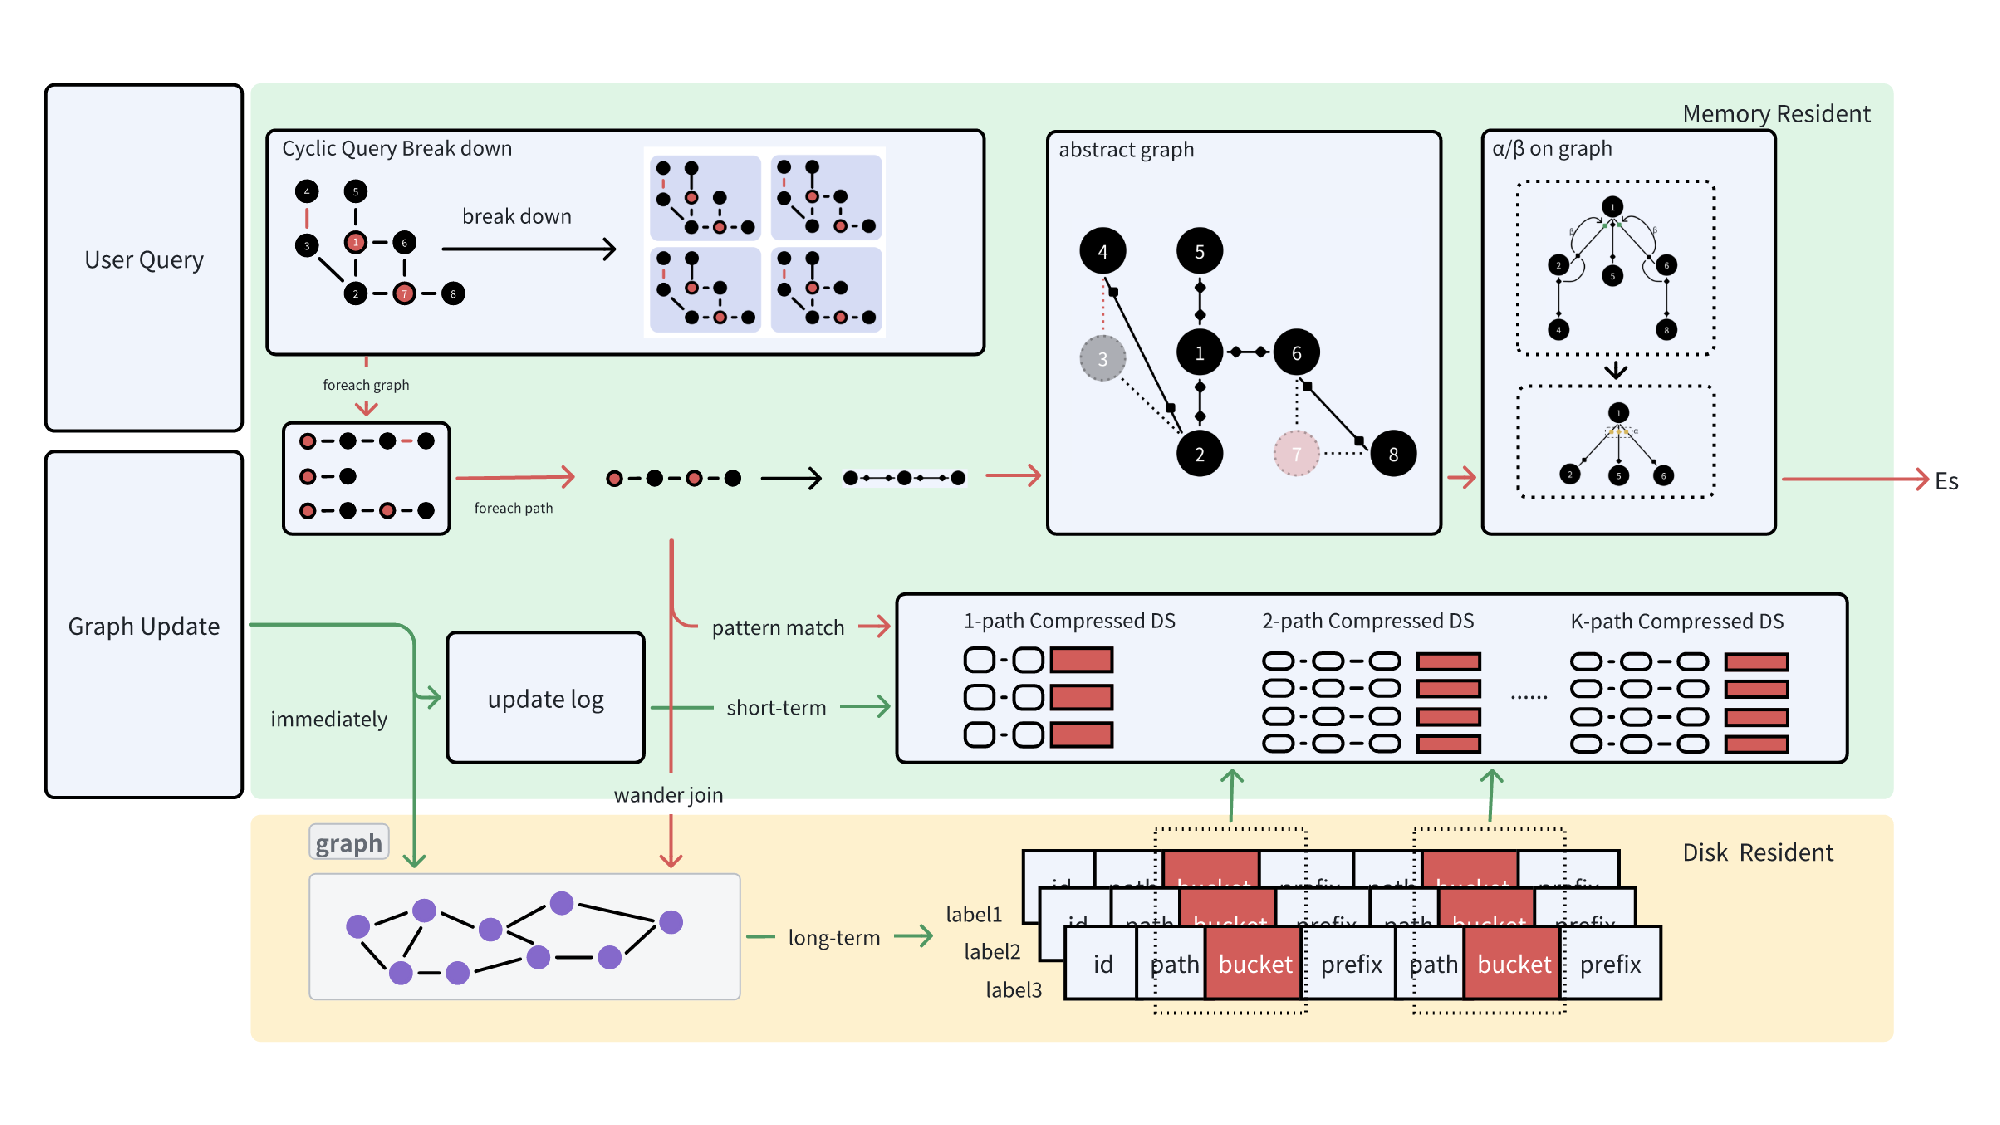
\includegraphics[width=\textwidth]{figures/sec-framework/framework_v1.pdf}
  \caption{Overview of GCard.}
  \label{fig:overview}
\end{figure*}

\stitle{PathDS: An Update-Friendly Summary}. \eat{At the core of GCard is
PathDS, a compact summary of path-level degree statistics. For each
degree value $d$, PathDS stores only a short high-order bit prefix
(e.g., 4 or 8 bits) and the highest-bit position, rather than the full
64-bit integer. During inference, GCard reconstructs a conservative value
$\hat d$ from this code such that $\hat d \ge d$, preserving an upper-bound
view of degree statistics. Because each update only changes the local
codes of affected paths, PathSketch supports efficient incremental
maintenance without rebuilding all summaries.}


\stitle{A Predicate Decoupling Design}. \eat{A key design principle of GCard
is predicate decoupling. Instead of materializing many
predicate-conditioned summaries offline, GCard keeps one structural
PathSketch and estimates predicate effects online as path-attached
selectivity factors. This design separates structural maintenance from
predicate handling, so data updates trigger only structural summary
updates, while predicate selectivity is evaluated at query time using a
conservative correction strategy.}

\stitle{A Cycle-Aware Estimation Algorithm}. \eat{For cyclic queries, GCard
first rewrites the query into an acyclic surrogate by removing a small
set of cycle-closing edges selected by a lightweight rule. It then
estimates the acyclic core with PathSketch and applies a conservative
recovery factor for the removed edges. This cycle-to-acyclic pipeline
keeps inference tractable while retaining conservative estimates on
cyclic workloads.}

\section{Handling Predicates}
\label{sec:predicate}

\section{PathDS Build and Maintenance}
\label{sec:pds}

In this section, we present a parallelly scalable construction algorithm
for PathDS and an efficient incremental update strategy.



\begin{algorithm}[t!]
  \caption{\kw{PDSBuild}: Parallel PathDS Construction}
  \label{alg:pds-build}
  \SetKwFunction{match}{Match} \SetKwFunction{extend}{Extend}
  \SetKwProg{Fn}{Procedure}{}{}
  \SetKwFunction{match}{Match}
  \SetKwFunction{init}{Init}
  \SetKwFunction{hs}{HSplit}
  \SetKwFunction{ts}{TSplit}
  \SetKwFunction{comp}{Compress}
  \SetKwFunction{getP}{GetsSubPaths}
  \SetKwFunction{maxlen}{MaxLen}
  \SetKwFor{ParaFor}{for each}{do in parallel}{endfor}
  \SetKwFor{ForEach}{for each}{do}{endfor}
  \SetKwComment{KwComment}{\# }{} %%
  \KwIn{Graph $G = (V,E,L)$, a set of path queries $\mathbb{P}$}%%
  \KwOut{PathDS $(\mathcal{S}_s^P, \mathcal{S}_t^P)$ for all $P\in\mathbb{P}$}

  $K \gets \maxlen(\mathbb{P})$; \ \ \
  $\{\mathbb{P}_1, \dots, \mathbb{P}_K\} \gets \getP(\mathbb{P}, K)$; 

  %\ParaFor{$v \in V,\, P \in \mathbb{P}$}{\init{$d_s^P(v), d_t^P(v)$}}
  Initialize $d_s^P(v), d_t^P(v)$ for all $v\in V$ and $P\in\mathbb{P}$;

  \ForEach{$i =1,\dots, K$}{

    \ForEach{$P \in \mathbb{P}_i$}{
      $(s,s', P_1) \gets \hs(P)$; \, \, $(P_2, t', t)\gets \ts(P)$;
      
      \ParaFor{$v\in V$}{
        %  $d_s^P(v) {\gets} \sum\bigl\{ d_{s'}^{P_1}(u)\mid u\in \kw{Nbr}(v),\,\match{v,u,s,s'}\bigr\}$

        % $d_t^P(v) {\gets} \sum\bigl\{ d_{t'}^{P_2}(u)\mid u\in \kw{Nbr}(v),\,\match{u,v,t',t}\bigr\}$
      
        Compute $d_s^P(v)$ and $d_t^P(v)$ via  Eqs.~(\ref{eq:dsP}) \& (\ref{eq:dtP})\;
      \lIf{$P \in \mathbb{P}$}{
        $\operatorname{Update}(\mathcal{S}_s^P, \mathcal{S}_t^P,d_s^P(v),d_t^P(v))$
      } %% IF
      }
    }%% ForEach
  
  }%% ForEach
  
  \Return{$\{(\mathcal{S}_s^P, \mathcal{S}_t^P)\}_{P\in\mathbb{P}}$};
\end{algorithm}

\subsection{Parallel PathDS Construction}\label{susbsec:pds-build}
\eat{
  1、介绍 PDSBuild 的设计原则和核心思想
  - 至底向上构建 flat path degrees
  - 算法并行的粒度，以点为中心进行并行
  2、给出算法1的描述，用文字的描述算法的流程和关键步骤
  3、分析算法的时间和空间复杂度，说明其并行效率和可扩展性
}

We first present \kw{PDSBuild}, a parallel algorithm that constructs
PathDS summaries for a given graph  and a set of path queries .

\vspace{.25em} %%
In a nutshell, \kw{PDSBuild} computes path degrees in bottom-up
manner and updates the corresponding PathDS summaries during the process.
%% 
The algorithm is parallelly scalable in the sense that it guarantees
reduced running time with more processing cores, enabling efficient
PathDS construction on large graphs.



\stitle{Bottom-Up Computation of Path Degrees.} %%
Given a path query $P$, we need the path degrees $(D_s^P, D_t^P)$ to
construct the corresponding PathDS  $(\mathcal{S}_s^P,
\mathcal{S}_t^P)$. %%
A key observation is that $(D_s^P, D_t^P)$ can be derived from the
path degrees of immediate sub-paths, which yields a bottom-up dynamic
construction from shorter paths to longer ones. Let $P=u_0e_1u_1\cdots
e_ku_k$, and define
$\kw{HSplit}(P)=(s,s',P_1)$ and $\kw{TSplit}(P)=(P_2,t',t)$, where
$s=u_0$, $t=u_k$, $s'=u_1$, $t'=u_{k-1}$, $P_1=u_1e_2\cdots e_ku_k$, and
$P_2=u_0e_1\cdots e_{k-1}u_{k-1}$. Then, for each vertex $v\in V$, its
path degrees \wrt $P$ can be computed as follows:
\begin{eqnarray}
  d_s^{P}(v) & = &\sum\bigl\{ d_{s'}^{P_1}(u)\mid u\in
  \kw{Nbr}(v),\,\kw{Match}(v,u,s,s')\bigr\}, \label{eq:dsP}\\
  d_t^{P}(v) & = &\sum\bigl\{ d_{t'}^{P_2}(u)\mid u\in \kw{Nbr}(v),\,\kw{Match}(u,v,t',t)\bigr\}. \label{eq:dtP}
\end{eqnarray}
Here, $\kw{Nbr}(v)$ denotes the set of neighbors of $v$ in $G$, and
$\kw{Match}(v,u,s,s')$ (resp. $\kw{Match}(u,v,t',t)$) checks whether the
data edge is compatible with the corresponding query edge in $P$.
Equations~\eqref{eq:dsP} and \eqref{eq:dtP} therefore reduce the
computation of $(D_s^P, D_t^P)$ to previously computed degrees on $P_1$
and $P_2$. 

\stitle{Parallel Processing.} %%
The path degree computation admits two-level parallelism. We can
process query groups by increasing path length, execute queries within
each group in parallel, and parallelize vertex-wise path degrees for
each query since they are independent given shorter-path results.



\stitle{Algorithm \kw{PDSBuild}}. %%
Putting these together, Algorithm~\ref{alg:pds-build} outlines the
PathDS construction procedure. %
Given a graph $G$ and a set of short path
queries $\mathbb{P}$, \kw{PDSBuild} constructs the corresponding PathDS
summaries $\{(\mathcal{S}_s^P, \mathcal{S}_t^P)\}_{P\in\mathbb{P}}$ for
all $P\in\mathbb{P}$ in parallel. 

\sstab (1) \kw{PDSBuild} first generates all sub-paths of queries in
$\mathbb{P}$ and groups them by length into
$\mathbb{P}_1,\dots,\mathbb{P}_K$ (line~1). %
It then initializes $d_s^P(v)$ and
$d_t^P(v)$ for all $v\in V$ and $P\in\mathbb{P}$ (line~2).

\sstab (2) \kw{PDSBuild} next computes the path degrees in a
bottom-up manner and in parallel (lines~4--7). For each
$P\in\mathbb{P}_i$, it applies $\kw{HSplit}/\kw{TSplit}$ to obtain the
sub-paths of $P$ and, in parallel over each vertex $v\in V$, computes
 $d_s^P(v),d_t^P(v)$ using  Eqs.~\eqref{eq:dsP}--\eqref{eq:dtP}. 

\sstab (3) When $P\in\mathbb{P}$, the computed degrees are mapped to
their ranks and used to update the corresponding rank buckets in the
PathDS summaries defined in Definition~\ref{def:pathds} (line~8).
It the end, \kw{PDSBuild} returns
$\{(\mathcal{S}_s^P,\mathcal{S}_t^P)\}_{P\in\mathbb{P}}$ (line~9).

\stitle{Analysis}. \todo{analyze the time and space complexity of \kw{PDSBuild}}

\subsection{Incremental PathDS Maintenance}\label{susbsec:pds-maintenance}

\plan{
1. 给出增量更新算法的问题定义
2. 介绍增量更新算法的挑战： pathDS 难以直接更新 
  --> 观察： 中间结果 path degrees 是可以增量更新 
  --> 基于观察给出基础方法：
      - 离线存储 path degrees DS, 基于 G, \delta G, 计算 \delta DS 
      - 给出代代码描述流程，参考 Sec 6.1
      - 分析算法的时间复杂度，说明其效率和适用场景
3. 指出基础方法的不足：需要存储全量 path degrees; 且更新效率受 path length 和 graph size 影响
4. 提出优化方法，说明优化方法的性能
}
\newpage

\label{subsec:flatr} a path pattern $P$, FlatDS records the exact number of matches of
$P$ originating from each valid start vertex.
Conceptually, FlatDS corresponds to the most fine-grained statistic
that PathDS can maintain and serves as the reference point for
subsequent compression.

\stitle{Collection Strategy.} [To be filled: description of how FlatDS is collected efficiently for each path pattern $P$, including traversal strategy ...etc].


\subsection{CompressedDS: Design and Representation}
\label{subsec:compress}

While FlatDS provides exact path statistics, it requires storing one
count per start vertex.
For large graphs or multiple path patterns, this results in substantial
space overhead, making it impractical as a maintained summary.

A natural compression strategy is to construct a compact summary
of FlatDS based on its ordered or aggregated distribution.
Such approaches derive their representation from the globally
arranged sequence of counts and often rely on cumulative
relationships among values.

While this can produce concise summaries, the resulting structure
exhibits cumulative dependencies: the representation of one position
is influenced by other values in the ordered sequence.
Consequently, a local modification may affect more than the modified
count itself, potentially requiring adjustments beyond the changed
value.

CompressedDS adopts a different design principle.
Instead of aggregating multiple entries into a shared statistic,
it compresses each FlatDS entry independently.


\stitle{Compression Procedure.} CompressedDS is constructed by applying entry-wise upper-bound compression to FlatDS.
For each exact count $x$, the compression produces a compact descriptor
$(\pi, k)$, where $k = \lceil \log_b x \rceil$ denotes the logarithmic
bucket index under base $b$, and $\pi$ stores the top-$n$ most
significant bits of $x$.
This representation preserves the order of magnitude of each entry
while reducing storage overhead.

For each bucket $k$, we also record the maximum exact value
$M_k$ among all path counts assigned to that bucket.
During cardinality estimation, all values mapped to bucket $k$
are conservatively approximated by $M_k$.

\begin{algorithm}[t]
\caption{FastCompress: Constructing CompressedDS}
\label{alg:fastcompress}
\KwIn{FlatDS $f_P = [x_1, x_2, \ldots, x_m]$, bucket base $b$, prefix length $n$}
\KwOut{CompressedDS $H$ and bucket maxima $\{M_k\}$}

\ForEach{$x \in f_P$}{
  $k \leftarrow \lceil \log_b x \rceil$\;
  $\pi \leftarrow$ top-$n$ most significant bits of $x$\;
  Insert $(\pi, k)$ into $H$\;
  $M_k \leftarrow \max(M_k, x)$\;
}
\Return{$H$ and $\{M_k\}$}
\end{algorithm}

Algorithm~\ref{alg:fastcompress} presents the construction procedure.
Because the algorithm scans FlatDS once and processes each entry independently,
FastCompress runs in linear time in $|f_P|$ and supports streaming
and parallel execution.
Its cost is insensitive to the global distribution of path counts,
and no cross-entry aggregation is required.


\begin{figure}[t]
  \centering
  % Placeholder for CompressedDS layout illustration
  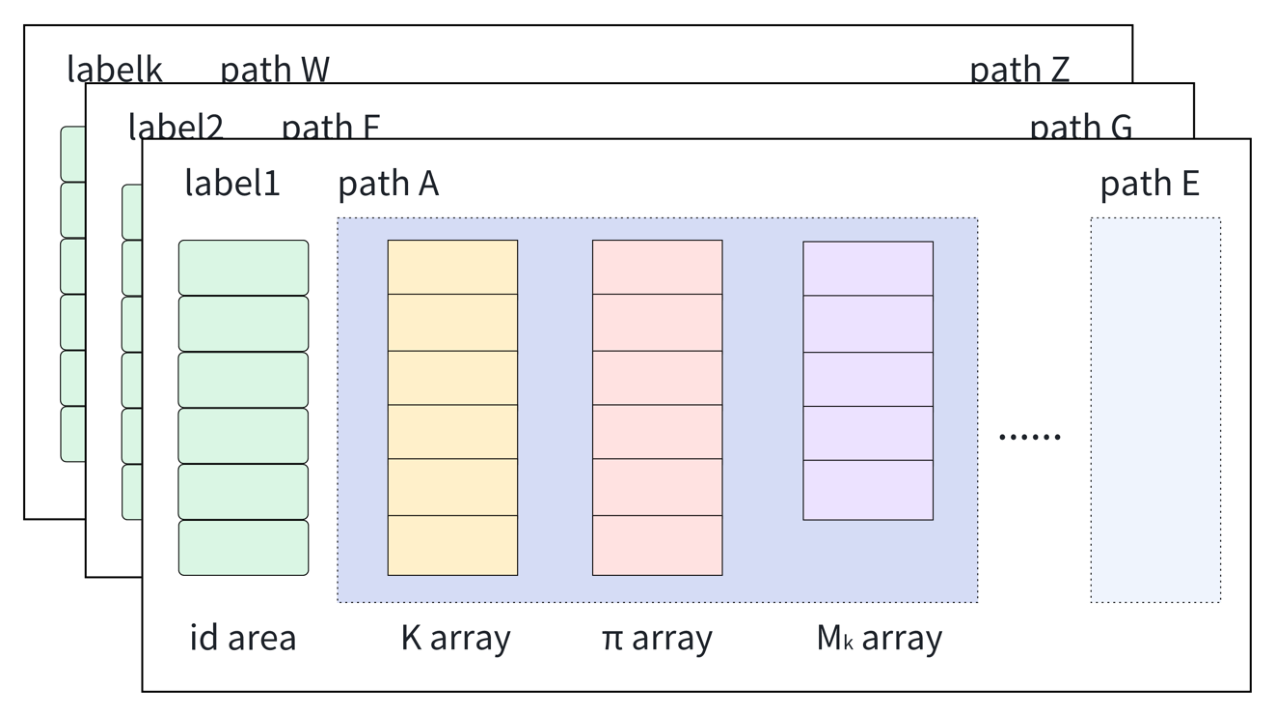
\includegraphics[width=\columnwidth]{figures/sec-pds/CompressedDS_memory_layout.pdf}
  % \fbox{\parbox{0.8\linewidth}{\centering
  % CompressedDS memory layout illustration}}
  \caption{In-memory representation of CompressedDS.}
  \label{fig:compressed_layout}
\end{figure}

\stitle{Memory Layout.} [To be filled:
CompressedDS is stored as a contiguous array of fixed-size entries
representing $(\pi, k)$ pairs.
Bucket-level maxima $\{M_k\}$ are stored in a separate compact array,
indexed by bucket identifier.
This separation allows efficient access to both per-entry information
and bucket metadata while maintaining cache-friendly memory access
patterns.]

\subsection{Incremental Updates}
\label{subsec:update}

With CompressedDS, path count changes can be handled incrementally.
Since compression is independent across path counts, an update
affects only the associated descriptor and its bucket metadata,
without requiring global reconstruction.

When the exact count of a path instance changes by a small value
$\Delta$, the corresponding compressed entry $(\pi, k)$ is updated as
follows.
First, we recover an estimate of the original
value using the current bucket maximum $M_k$.
Specifically, the value is restored as $x = M_k$.
After applying the update, the new value $x' = x + \Delta$ is mapped to a
possibly new bucket $k' = \lceil \log_b x' \rceil$, and a new prefix
$\pi'$ is extracted accordingly.

If $k' = k$, the update does not change the order of magnitude of the
value, and no bucket migration is required.
Only the bucket maximum $M_k$ is updated if $x'$ exceeds the current
maximum.
If $k' \neq k$, the entry migrates to the new bucket $k'$, and both
$M_k$ and $M_{k'}$ are updated accordingly.

This update strategy ensures that each modification affects only
constant-sized metadata,
resulting in amortized constant update cost while preserving
the upper-bound guarantee.



\subsection{Upper-Bound Correctness and Estimation Accuracy}
\label{subsec:theory}

\stitle{Upper-Bound Preservation.}
[proof]

\stitle{Estimation Accuracy.}
[proof]

\newpage
\section{Handling Cycles}
\label{sec:cycle}


\section{Evaluation}\label{sec:eval}

\stitle{Experimental settings}. We start with experimental settings.

\etitle{Datasets and Queries}.

\begin{figure*}[tb!]
  \vspace{-1.7ex}
  \begin{center}
    \begin{minipage}[t]{\textwidth}

      \begin{subfigure}[b]{0.24\textwidth}
        
\includegraphics[width=\textwidth]{exp/blank.eps}
        \caption{Scalability (vary thread count)}
        \label{fig:scale-thread}
      \end{subfigure}
      \vspace{.4em}
      \hfill
      \begin{subfigure}[b]{0.24\textwidth}
        
\includegraphics[width=\textwidth]{exp/blank.eps}
        \caption{Scalability (vary scale factor)}
        \label{fig:scale-graph}
      \end{subfigure}
      \hfill
      \begin{subfigure}[b]{0.24\textwidth}
        
\includegraphics[width=\textwidth]{exp/blank.eps}
        \caption{End-to-end evaluation (\ldbc)}
        \label{fig:e2e-ldbc}
      \end{subfigure}
      \hfill
      \begin{subfigure}[b]{0.24\textwidth}
        
\includegraphics[width=\textwidth]{exp/blank.eps}
        \caption{End-to-end evaluation (\imdb)}
        \label{fig:e2e-imdb}
      \end{subfigure}


            \begin{subfigure}[b]{0.24\textwidth}
        
\includegraphics[width=\textwidth]{exp/blank.eps}
        \caption{Scalability (vary thread count)}
        \label{fig:scale-thread}
      \end{subfigure}
      \vspace{.4em}
      \hfill
      \begin{subfigure}[b]{0.24\textwidth}
        
\includegraphics[width=\textwidth]{exp/blank.eps}
        \caption{Scalability (vary scale factor)}
        \label{fig:scale-graph}
      \end{subfigure}
      \hfill
      \begin{subfigure}[b]{0.24\textwidth}
        
\includegraphics[width=\textwidth]{exp/blank.eps}
        \caption{End-to-end evaluation (\ldbc)}
        \label{fig:e2e-ldbc}
      \end{subfigure}
      \hfill
      \begin{subfigure}[b]{0.24\textwidth}
        
\includegraphics[width=\textwidth]{exp/blank.eps}
        \caption{End-to-end evaluation (\imdb)}
        \label{fig:e2e-imdb}
      \end{subfigure}

            \begin{subfigure}[b]{0.24\textwidth}
        
\includegraphics[width=\textwidth]{exp/blank.eps}
        \caption{Scalability (vary thread count)}
        \label{fig:scale-thread}
      \end{subfigure}
      \vspace{.4em}
      \hfill
      \begin{subfigure}[b]{0.24\textwidth}
        
\includegraphics[width=\textwidth]{exp/blank.eps}
        \caption{Scalability (vary scale factor)}
        \label{fig:scale-graph}
      \end{subfigure}
      \hfill
      \begin{subfigure}[b]{0.24\textwidth}
        
\includegraphics[width=\textwidth]{exp/blank.eps}
        \caption{End-to-end evaluation (\ldbc)}
        \label{fig:e2e-ldbc}
      \end{subfigure}
      \hfill
      \begin{subfigure}[b]{0.24\textwidth}
        
\includegraphics[width=\textwidth]{exp/blank.eps}
        \caption{End-to-end evaluation (\imdb)}
        \label{fig:e2e-imdb}
      \end{subfigure}

            \begin{subfigure}[b]{0.24\textwidth}
        
\includegraphics[width=\textwidth]{exp/blank.eps}
        \caption{Scalability (vary thread count)}
        \label{fig:scale-thread}
      \end{subfigure}
      \vspace{.4em}
      \hfill
      \begin{subfigure}[b]{0.24\textwidth}
        
\includegraphics[width=\textwidth]{exp/blank.eps}
        \caption{Scalability (vary scale factor)}
        \label{fig:scale-graph}
      \end{subfigure}
      \hfill
      \begin{subfigure}[b]{0.24\textwidth}
        
\includegraphics[width=\textwidth]{exp/blank.eps}
        \caption{End-to-end evaluation (\ldbc)}
        \label{fig:e2e-ldbc}
      \end{subfigure}
      \hfill
      \begin{subfigure}[b]{0.24\textwidth}
        
\includegraphics[width=\textwidth]{exp/blank.eps}
        \caption{End-to-end evaluation (\imdb)}
        \label{fig:e2e-imdb}
      \end{subfigure}
    \end{minipage}
  \end{center}
  \vspace{-3.4ex}
  \caption{Performance Evaluation}
  \vspace{-1.7ex}
  \label{fig:eval}
\end{figure*}

\etitle{Environment}.

\vspace{-.3em}
\stitle{Exp-1: Estimation Accuracy}.

\stitle{Exp-2: Estimation Latency}.

\stitle{Exp-3: PDS Construction Latency}.

\stitle{Exp-4: PDS Maintenance Efficiency}.

\stitle{Exp-5: Scalability of DS Construction}.

\stitle{Exp-6: Micro Benchmarks}.


\stitle{Exp-6: Impact On End-to-End Performance}.
\newpage
\section{Conclusion}\label{sec:conclude}



\bibliographystyle{ACM-Reference-Format}
\bibliography{ref}
\end{document}
\endinput

%%% Local Variables:
%%% mode: latex
%%% TeX-master: t
%%% End:
